% This presentation is based on a Beamer theme from Seth Brown, distributed
% under the following license:
%
% ----------------------------------------------------------------------------
% This program can be redistributed and/or modified under the terms
% of the GNU Public License, version 3.
%
% Seth Brown, Ph.D.
% sethbrown@drbunsen.org

\documentclass[t,aspectratio=169]{beamer}

%\usepackage{xcolor}

% White on black scheme
\definecolor{lightbg}{HTML}{808080}     % 50% gray
\definecolor{mediumbg}{HTML}{666666}    % 60% gray
\definecolor{darkbg}{HTML}{333333}      % 80% gray
\definecolor{background}{HTML}{1A1A1A}  % 90% gray
\definecolor{foreground}{HTML}{FFFFFF}  % white

\definecolor{active1}{HTML}{FFE499}     % pale orange
\definecolor{active2}{HTML}{FF99FF}     % pale pink
\definecolor{active3}{HTML}{00FFFF}     % cyan

%\usepackage{xcolor}

% "chalkboard" scheme
%
% def mix(ac,bc,f): return "#%02X%02X%02X" % tuple([int((a * float(f)) + (b * (1.0 - f))) for a,b in zip(ac, bc)])

\definecolor{lightbg}{HTML}{AEC2B4}     % 40% tint of chalkboard green
\definecolor{mediumbg}{HTML}{153E29}
\definecolor{darkbg}{HTML}{1A3422}      % 50% shade of chalkboard green
\definecolor{background}{HTML}{356845}  % Chalkboard green
\definecolor{foreground}{HTML}{FFFFFF}  % white

\definecolor{active1}{HTML}{FAD48B}     % Orange Chalk
\definecolor{active2}{HTML}{BCDF8A}     % Green Chalk
\definecolor{active3}{HTML}{94C0CC}     % Blue Chalk

\usepackage{xcolor}

% "chalkboard" scheme
%
% def mix(ac,bc,f): return "#%02X%02X%02X" % tuple([int((a * float(f)) + (b * (1.0 - f))) for a,b in zip(ac, bc)])

%\definecolor{lightbg}{HTML}{ABB8B8}     % 40% tint of Dark Slate Gray
%\definecolor{lightbg}{HTML}{829595}     % 60% tint of Dark Slate Gray
\definecolor{lightbg}{HTML}{778899}     % Light Slate Gray
\definecolor{mediumbg}{HTML}{253F3F}    % 80% shade of Dark Slate Gray
\definecolor{darkbg}{HTML}{172727}      % 50% shade of Dark Slate Gray
\definecolor{background}{HTML}{2F4F4F}  % Dark Slate Gray
\definecolor{foreground}{HTML}{FFFFFF}  % white

% http://designpieces.com/2014/02/chalkboard-look-and-feel/
%\definecolor{active1}{HTML}{FAD48B}     % Orange Chalk
%\definecolor{active2}{HTML}{BCDF8A}     % Green Chalk
%\definecolor{active2}{HTML}{ED7777}     % Red Chalk
%#\definecolor{active2}{HTML}{F2A3BD}     % Pink Chalk
%\definecolor{active3}{HTML}{94C0CC}     % Blue Chalk
%\definecolor{active3}{HTML}{6FE7DB}     % Turquoise Chalk

\definecolor{active1}{HTML}{FAD48B}     % Orange Chalk
\definecolor{active2}{HTML}{FF99FF}     % Pale Pink
%\definecolor{active3}{HTML}{00FFFF}     % Cyan
\definecolor{active3}{HTML}{2FF4F4}     % ~80% tint of Cyan

\mode<presentation>{\usetheme{codeplay}}

% title slide definition
\title{Creating an SPMD Vectorizer for OpenCL with LLVM}
\subtitle{LLVM 2015 Tutorial}
\author{Pierre-André Saulais \\ <pierre-andre@codeplay.com>}
\institute{Codeplay Software \\ @codeplaysoft}

\date{October 29, 2015}

\newcommand{\varying}[1]{\codeempha{#1}}
\newcommand{\uniform}[1]{\codeemphb{#1}}
\newcommand{\glossaryword}[2]{\textbf{#1}: #2}

\newcommand{\pointfor}[1]{\hspace{1em}\textbf{\codeemphb{{\fontspec{Cambria Math} +}}}\hspace{0.5em}#1}
\newcommand{\pointunkn}[1]{\hspace{1em}\textbf{?}\hspace{0.5em}#1}
\newcommand{\pointagainst}[1]{\hspace{1em}\textbf{\codeempha{{\textendash}}}\hspace{0.5em}#1}

\newcommand{\llvmlogo}[1]{\raisebox{-1.3ex}{
\includegraphics[scale=#1]{images/LLVM_Logo.pdf}}\hspace{-0.3em}}
\newcommand{\llvmlogovec}[1]{\llvmlogo{#1}, \llvmlogo{#1}, \llvmlogo{#1}, \llvmlogo{#1}, \llvmlogo{#1}, \llvmlogo{#1}, \llvmlogo{#1}, \llvmlogo{#1}\hspace{0.3em}}

\newcommand{\fullpagediagram}[2]{\hfill\includegraphics[scale=#1]{#2}\hfill\hfill}

%%%%%%%%%%%%%%%%%%%%%%%%%%%%%%%%%%%%%%%%%%%%%%%%%%%%%%%%%%%%%%%%%%%%%%%%%%%%%%%%

\begin{document}

%\setbeamertemplate{background}
%{
\includegraphics[width=\paperwidth,height=\paperheight]{dark_background_title.png}}
\setbeamertemplate{footline}[default]

\begin{frame}
  \vspace{4ex}
  \titlepage
\end{frame}

%%%%%%%%%%%%%%%%%%%%%%%%%%%%%%%%%%%%%%%%%%%%%%%%%%%%%%%%%%%%%%%%%%%%%%%%%%%%%%%%

\setbeamertemplate{background}{}
\setbeamertemplate{footline}[codeplaytheme]

\section*{Introduction}

\begin{frame}{What this tutorial is about}

\begin{minipage}[t]{0.70\linewidth}

\begin{itemize}  
    \item Vectorizing
    \begin{itemize}
        \item Transform whole functions using LLVM
        \item "Horizontal" vectorization (not loop-based)
    \end{itemize}  
    \item SPMD (Single Program, Multiple Data) Kernels
    \begin{itemize}
        \item Data-parallel execution model
        \item Compute frameworks like OpenCL\textsuperscript{TM} and CUDA\textsuperscript{TM}
    \end{itemize}
    \item for CPUs, DSPs,
    \begin{itemize}
        \item Explicitly programmed SIMD unit(s)
        \item Can execute both scalar and vector instructions
    \end{itemize}
    \item An introduction
    \begin{itemize}
        \item Create a basic vectorizer
    \end{itemize}
\end{itemize}

\end{minipage}\hspace{1em}\begin{minipage}[t]{0.25\linewidth}
\vspace{-3.5ex}
\center{
\includegraphics[scale=0.07]{images/LLVM_Logo.pdf}}
\vspace{-2.5ex}\center{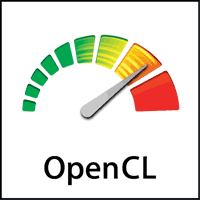
\includegraphics[scale=0.25]{images/OpenCL_Logo.png}}
\center{
\includegraphics[scale=0.155]{images/CUDA.png}}

\end{minipage}

\end{frame}

%%%%%%%%%%%%%%%%%%%%%%%%%%%%%%%%%%%%%%%%%%%%%%%%%%%%%%%%%%%%%%%%%%%%%%%%%%%%%%%%

\begin{frame}{Overview}
\tableofcontents
\end{frame}

%%%%%%%%%%%%%%%%%%%%%%%%%%%%%%%%%%%%%%%%%%%%%%%%%%%%%%%%%%%%%%%%%%%%%%%%%%%%%%%%

\talkpart{1}{Background}
%%%%%%%%%%%%%%%%%%%%%%%%%%%%%%%%%%%%%%%%%%%%%%%%%%%%%%%%%%%%%%%%%%%%%%%%%%%%%%%%

\begin{frame}{SPMD execution model}

\end{frame}


%% Kernel function has no return value, takes in buffers (arrays)
%% Vectorization does not change the signature for kernels
%% Can also vectorize "normal" functions, but this results in signature changes


\talkpart{2}{Implementing a SPMD Vectorizer}
%%%%%%%%%%%%%%%%%%%%%%%%%%%%%%%%%%%%%%%%%%%%%%%%%%%%%%%%%%%%%%%%%%%%%%%%%%%%%%%%

\talksection{Overview}

\begin{frame}{Structure}

\begin{itemize}
    \item Pipeline design
    \begin{itemize}
        \item $F$ is repeatedly transformed by different stages
        \item Stages are independent from each other
        \item Each stage consists of one or more IR passes
        \item Most stages require some analysis
    \end{itemize}
    \item Analyses
    \begin{itemize}
        \item Capture information about the IR to vectorize
        \item May need updating after a stage (stale information)
        \item May depend on other analyses
    \end{itemize}
\end{itemize}

\center{
\includegraphics[width=0.8\textwidth]{images/stages.pdf}}

\end{frame}

%%%%%%%%%%%%%%%%%%%%%%%%%%%%%%%%%%%%%%%%%%%%%%%%%%%%%%%%%%%%%%%%%%%%%%%%%%%%%%%%

\begin{frame}{Analysis Examples}

\begin{itemize}
    \item Uniform Value Analysis
    \begin{itemize}
        \item Marks values as either \uniform{uniform} or \varying{varying}
    \end{itemize}

    \item Control Flow Analysis
    \begin{itemize}
        \item Determines which basic blocks are \varying{divergent}
        \item Builds a Control Dependency Graph
    \end{itemize}
    
    \item SIMD Width Analysis
    \begin{itemize}
        \item Chooses a 'good' width $N$ based on register/instruction usage
    \end{itemize}
    
    \item ...
\end{itemize}

\end{frame}

%%%%%%%%%%%%%%%%%%%%%%%%%%%%%%%%%%%%%%%%%%%%%%%%%%%%%%%%%%%%%%%%%%%%%%%%%%%%%%%%

\begin{frame}{Implementation Level: IR or MI?}

\begin{itemize}
    \item IR
        \\ \pointfor{Use-def graph and RAUW make for straightforward transformations}
        \\ \pointfor{Easy to target multiple platforms}
        \\ \pointunkn{Generally higher-level (simpler implementation?)}
        \\ \pointagainst{Platform-specific features more difficult to use}
        \\ \pointagainst{SIMD predication only for a few operations (select, load/stores)}

    \item MachineInstr (i.e. backend level)
        \\ \pointfor{Easy to use platform-specific features (e.g. predication, mask registers)}
        \\ \pointunkn{Generally lower-level (more powerful?)}
        \\ \pointagainst{More platform-specific code}
        \\ \pointagainst{Graph-based transformations not as straightforward}
    
\end{itemize}

\end{frame}

%%%%%%%%%%%%%%%%%%%%%%%%%%%%%%%%%%%%%%%%%%%%%%%%%%%%%%%%%%%%%%%%%%%%%%%%%%%%%%%%

%\begin{frame}{Implementation strategy}
%
%\begin{itemize}
%    \item Create test kernels
%    \begin{itemize}
%        \item Start with very simple kernels (e.g. copy buffer, add two buffers)
%        \item Gradually add more features (e.g. non-sequential memory accesses, vector instructions, etc)
%    \end{itemize}
%
%    
%    \item Suggested implementation order
%    \begin{itemize}
%        \item Preparation and packetization first (required for simplest kernels)
%        \item Then easier features: builtins, memory addressing, scalarization, instantiation
%        \item More complex features last: control flow, optimizations
%    \end{itemize}
%\end{itemize}
%
%\end{frame}

\talksection{Packetization Stage}

\begin{frame}{Packetization Overview}

\begin{itemize}
    \item Stage that does the actual vectorization: $<F, N> \rightarrow VF_N$
    \begin{itemize}
        \item Calling $VF_N$ is like calling $F$, but $N$ times ($N$: SIMD width)
        \item Straightforward thanks to preparation from previous stages
    \end{itemize}
    
    \item This is done per-instruction, for the whole function
    \begin{itemize}
        \item Instructions that define a value: define $N$ values, one for each instance
        \item Instructions with side effects: perform side effects for each instance
        %\item New instruction has the same opcode but different types
    \end{itemize}
    
    \item Only \varying{varying} instructions need packetization
    \begin{itemize}
        \item \uniform{Uniform} instructions can remain scalar, executed once per work-group
        \item Requires \emph{Uniform Value Analysis} to know which instructions to vectorize
    \end{itemize}
    
\end{itemize}

\vspace{1.5ex}
\hspace{1em}
\includegraphics[scale=0.55]{images/stages-packet.pdf}

\end{frame}

%%%%%%%%%%%%%%%%%%%%%%%%%%%%%%%%%%%%%%%%%%%%%%%%%%%%%%%%%%%%%%%%%%%%%%%%%%%%%%%%

\begin{frame}{Uniform Value Analysis}

\begin{itemize}
    \item Finds 'root' values
    \begin{itemize}
        \item \varying{Varying} values with no \varying{varying} operand
        \item Example: \varying{get\_global\_id(0)} has a different value for each isntance
    \end{itemize}
    \item Marks each IR value as \uniform{uniform} or \varying{varying}
    \begin{itemize}
        \item All values start as \uniform{uniform}
        \item Marking a value as \varying{varying} causes all users to also be marked \varying{varying}
        \item Marking is done recursively, starting with roots
        \item Values are marked before their users, to avoid cycles (phi nodes)
    \end{itemize}
\end{itemize}

\end{frame}

%%%%%%%%%%%%%%%%%%%%%%%%%%%%%%%%%%%%%%%%%%%%%%%%%%%%%%%%%%%%%%%%%%%%%%%%%%%%%%%%

\begin{frame}[fragile]{Uniform Value Analysis}

Example that combines \uniform{uniform} and \varying{varying} values:

\begin{codebox}[commandchars=\\\[\]]
kernel void add_uniform(global int *\uniform[dst], global int *\uniform[src], int \uniform[alpha]) {
    int \varying[tid] = \varying[get_global_id](0);
    \uniform[dst]\idx[\varying[tid]] = \uniform[src]\idx[\varying[tid]] + (\uniform[alpha] - \uniform[1]);
}
\end{codebox}

\begin{codebox}[commandchars=\\\[\]]
define void @add_uniform(i32* \uniform[%dst], i32* \uniform[%src], i32 \uniform[%alpha]) {
entry:
  \varying[%tid] = i32 \varying[@get_global_id(i32 0)]
  \varying[%arrayidx] = getelementptr i32* \uniform[%src], i32 \varying[%tid]
  \varying[%tmp] = load i32* \varying[%arrayidx], align 4
  \uniform[%sub] = sub i32 \uniform[%alpha], \uniform[1]
  \varying[%add] = add i32 \uniform[%sub], \varying[%tmp]
  \varying[%arrayidx2] = getelementptr i32* \uniform[%dst], i32 \varying[%tid]
  store i32 \varying[%add1], i32* \varying[%arrayidx2], align 4
  ret void
}
\end{codebox}

\end{frame}

%%%%%%%%%%%%%%%%%%%%%%%%%%%%%%%%%%%%%%%%%%%%%%%%%%%%%%%%%%%%%%%%%%%%%%%%%%%%%%%%

\begin{frame}[c]{UVA Example: Start}

\center{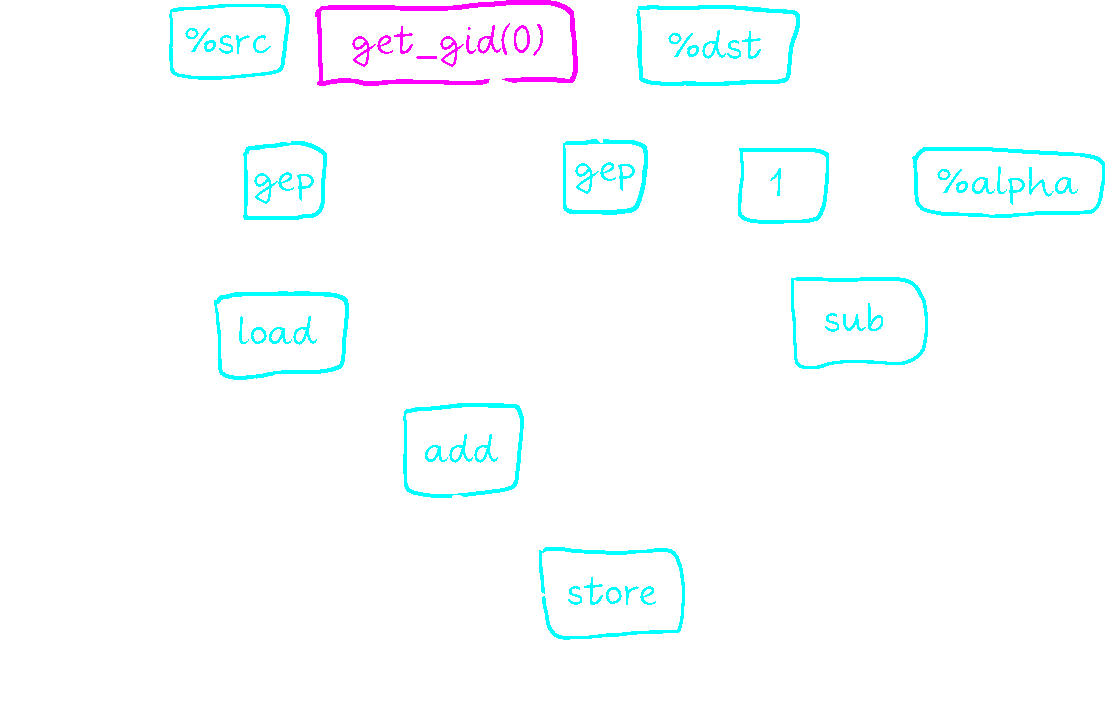
\includegraphics[scale=0.6]{images/uva-example-start.pdf}}

\end{frame}

%%%%%%%%%%%%%%%%%%%%%%%%%%%%%%%%%%%%%%%%%%%%%%%%%%%%%%%%%%%%%%%%%%%%%%%%%%%%%%%%

\begin{frame}[c]{UVA Example: Propagation}

\center{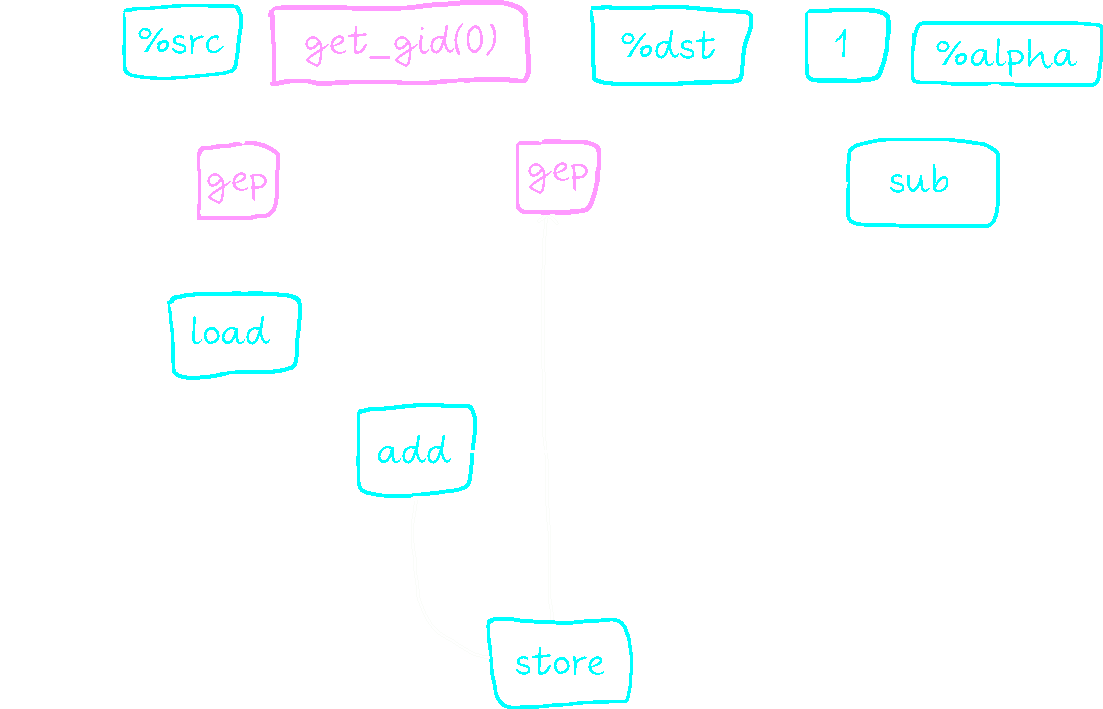
\includegraphics[scale=0.6]{images/uva-example-interm.pdf}}

\end{frame}

%%%%%%%%%%%%%%%%%%%%%%%%%%%%%%%%%%%%%%%%%%%%%%%%%%%%%%%%%%%%%%%%%%%%%%%%%%%%%%%%

\begin{frame}[c]{UVA Example: End}

\center{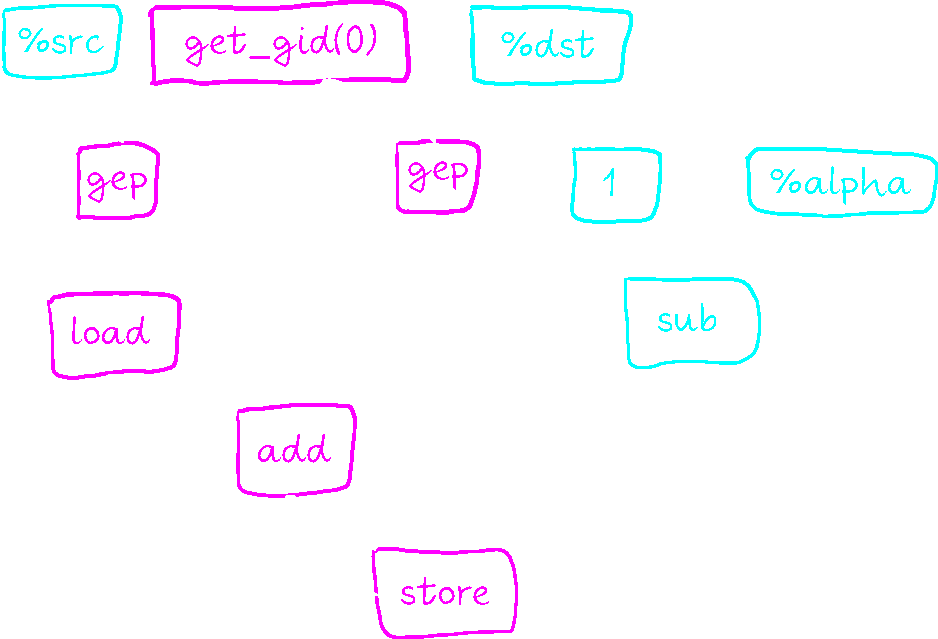
\includegraphics[scale=0.6]{images/uva-example-end.pdf}}

\end{frame}

%%%%%%%%%%%%%%%%%%%%%%%%%%%%%%%%%%%%%%%%%%%%%%%%%%%%%%%%%%%%%%%%%%%%%%%%%%%%%%%%

\begin{frame}{Memory Addressing}

\begin{itemize}
    %\item \varying{get\_global\_id(0)} was not packetized to a sequence of IDs. Why?
    \item Loads and stores are packetized according to the addressing mode
    \begin{itemize}
        \item Each operation can access $N$ memory elements
        \item Address usually has the form `\uniform{base} + \varying{offset}'
        \item Need to evaluate the offset for each of the $N$ lanes
    \end{itemize}
    
    \item How are these elements laid out in memory?
    \begin{itemize}
        \item The layout affects how operations are packetized
        \item Most common layouts can be described with a single \emph{stride}
    \end{itemize}
    
    \item Stride is the distance between successive elements
    \begin{itemize}
        \item Expressed in number of elements
        \item "How many elements are skipped in memory to get to the next one"
        \item One means elements are consecutive
        \item Negative means memory offsets are decreasing
    \end{itemize}
    
    %\item Not all kinds of memory operations can be expressed in IR
    %\begin{itemize}
    %    \item Generate calls to internal builtins
    %    \item Internal builtins can be implemented for each target as supported 
    %\end{itemize}
    
\end{itemize}

\end{frame}

%%%%%%%%%%%%%%%%%%%%%%%%%%%%%%%%%%%%%%%%%%%%%%%%%%%%%%%%%%%%%%%%%%%%%%%%%%%%%%%%

\begin{frame}[fragile]{Uniform Memory Addressing}

%% TODO: Use 1 as offset, update the diagram
\begin{itemize}
    \item Constant $Stride = 0$
    \item Packetized offset is \uniform{uniform} (e.g. $<0, 0, 0, 0>$)
    \item Transformed to a regular \emph{scalar} load or store
\end{itemize}

\begin{minipage}[t]{0.40\linewidth}
    \vspace{0.1ex}
    \begin{codebox}[commandchars=\\\[\]]

global int \uniform[*src];
int \uniform[x] = \uniform[src]\idx[\uniform[0]];






    \end{codebox}
\end{minipage}
\begin{minipage}[t]{0.49\linewidth}
    \begin{figure}
        
\includegraphics[scale=0.5]{images/uniform-access.pdf}
    \end{figure}
\end{minipage}

\end{frame}

%%%%%%%%%%%%%%%%%%%%%%%%%%%%%%%%%%%%%%%%%%%%%%%%%%%%%%%%%%%%%%%%%%%%%%%%%%%%%%%%

\begin{frame}[fragile]{Sequential Memory Addressing}

\begin{itemize}
    \item Constant $Stride = 1$
    \item Packetized offset is a sequence like $<0, 1, 2, 3>$
    \item Transformed to a regular \emph{vector} load or store
\end{itemize}

\begin{minipage}[t]{0.40\linewidth}
    \vspace{0.1ex}
    \begin{codebox}[commandchars=\\\[\]]

global int \uniform[*src];
int \varying[tid] = \varying[get_global_id(0)];
int \varying[x] = \uniform[src]\idx[\varying[tid]];





    \end{codebox}
\end{minipage}
\hspace{1em}
\begin{minipage}[t]{0.49\linewidth}
    \begin{figure}
        
\includegraphics[scale=0.5]{images/sequential-access.pdf}
    \end{figure}
\end{minipage}

\end{frame}

%%%%%%%%%%%%%%%%%%%%%%%%%%%%%%%%%%%%%%%%%%%%%%%%%%%%%%%%%%%%%%%%%%%%%%%%%%%%%%%%

\begin{frame}[fragile]{Interleaved Memory Addressing}

\begin{itemize}
    \item Constant $Stride > 1$
    \item Packetized offset is a sequence like $<0, 2, 4, 6>$
    \item Transformed to an \emph{interleaved} load or store
\end{itemize}

\begin{minipage}[t]{0.40\linewidth}
    \vspace{0.1ex}
    \begin{codebox}[commandchars=\\\[\]]
    
global int \uniform[*src];
int \varying[tid] = \varying[get_global_id(0)];
int \varying[even] = \uniform[src]\idx[\varying[tid] * \uniform[2]];
int \varying[odd] = \uniform[src]\idx[(\varying[tid] * \uniform[2]) + \uniform[1]];




    \end{codebox}
\end{minipage}
\hspace{1em}
\begin{minipage}[t]{0.49\linewidth}
    \begin{figure}
        
\includegraphics[scale=0.5]{images/interleaved-access.pdf}
    \end{figure}
\end{minipage}

\end{frame}

%%%%%%%%%%%%%%%%%%%%%%%%%%%%%%%%%%%%%%%%%%%%%%%%%%%%%%%%%%%%%%%%%%%%%%%%%%%%%%%%

\begin{frame}[fragile]{Arbitrary Memory Addressing}

\begin{itemize}
    \item Variable stride
    \item Packetized offset can be any sequence (e.g. $<0, 3, 7, 3>$)
    \item Transformed to a \emph{gather} load or \emph{scatter} store
\end{itemize}

\begin{minipage}[t]{0.40\linewidth}
    \vspace{0.1ex}
    \begin{codebox}[commandchars=\\\[\]]
    
global int \uniform[*src];
global int \uniform[*map];
int \varying[tid] = \varying[get_global_id(0)];
int \varying[x] = \uniform[src]\idx[\uniform[map]\idx[\varying[tid]]];




    \end{codebox}
\end{minipage}
\hspace{1em}
\begin{minipage}[t]{0.49\linewidth}
    \begin{figure}
        
\includegraphics[scale=0.5]{images/arbitrary-access.pdf}
    \end{figure}
\end{minipage}

\end{frame}

%%%%%%%%%%%%%%%%%%%%%%%%%%%%%%%%%%%%%%%%%%%%%%%%%%%%%%%%%%%%%%%%%%%%%%%%%%%%%%%%

\begin{frame}{Packetization Process}

\begin{itemize}
    \item Find leaves
    \begin{itemize}
        \item Leaves allow \varying{varying} values to 'escape' from the function, they are:
        \item Store instructions (\varying{varying} operand)
        \item Call instructions (\varying{varying} operand, or call has no use)
        \item Return instructions
    \end{itemize}
\end{itemize}

\begin{itemize}
    \item Recursively packetize leaves and their operands
    \begin{itemize}
        \item Broadcast \uniform{uniform} values (e.g. argument, constants)
        \item Replace \varying{get\_global\_id(0)} with a vector of IDs
        \item Packetize operands first, then instruction (top-down)
        \item Cache packetized values to prevent duplication
    \end{itemize}
\end{itemize}

\begin{itemize}
    \item Delete original scalar instructions if dead
\end{itemize}

\end{frame}

%%%%%%%%%%%%%%%%%%%%%%%%%%%%%%%%%%%%%%%%%%%%%%%%%%%%%%%%%%%%%%%%%%%%%%%%%%%%%%%%

\begin{frame}[c]{Packetization Example}

\center{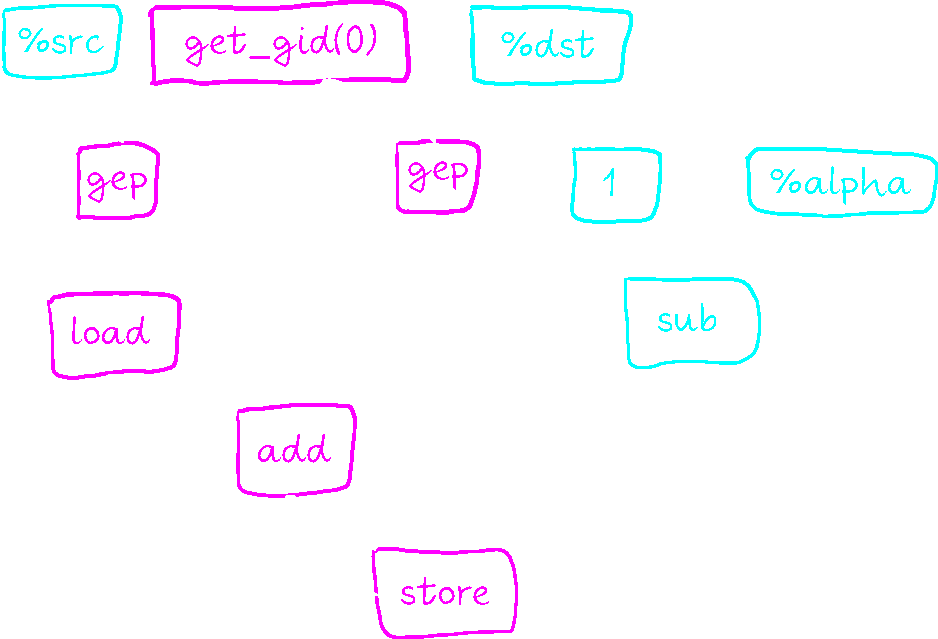
\includegraphics[scale=0.55]{images/uva-example-end.pdf}}

\end{frame}

%%%%%%%%%%%%%%%%%%%%%%%%%%%%%%%%%%%%%%%%%%%%%%%%%%%%%%%%%%%%%%%%%%%%%%%%%%%%%%%%

\begin{frame}[c]{Packetization Example}

\center{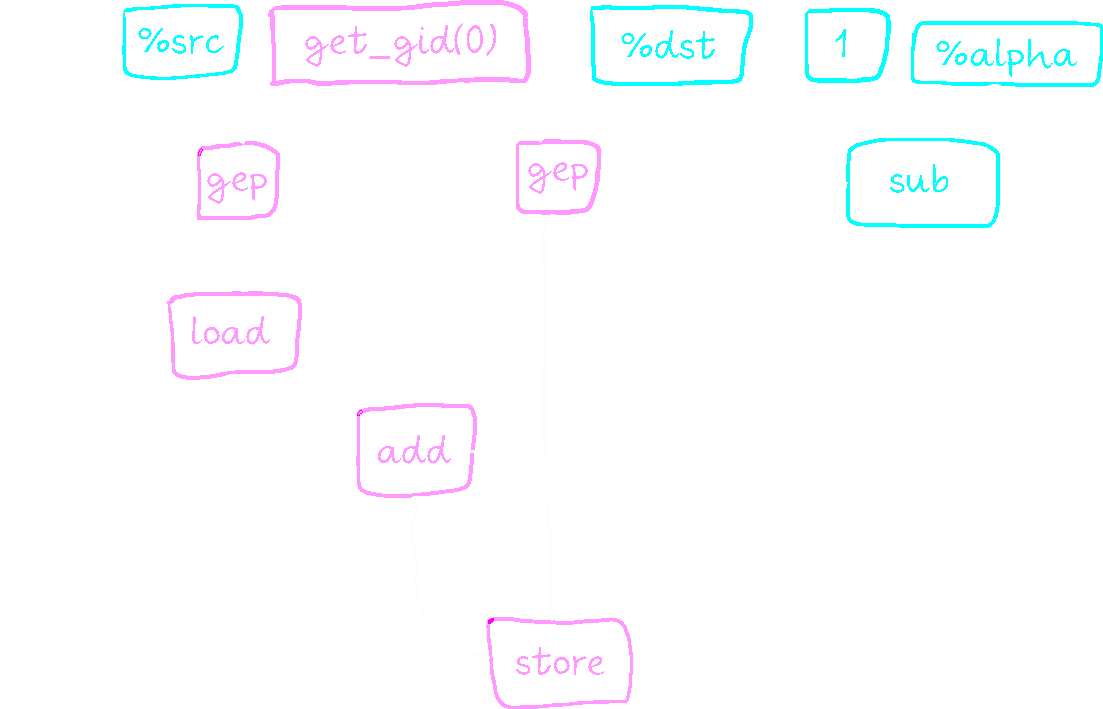
\includegraphics[scale=0.55]{images/packetization-1.pdf}}

\end{frame}

%%%%%%%%%%%%%%%%%%%%%%%%%%%%%%%%%%%%%%%%%%%%%%%%%%%%%%%%%%%%%%%%%%%%%%%%%%%%%%%%

\begin{frame}[c]{Packetization Example}

\center{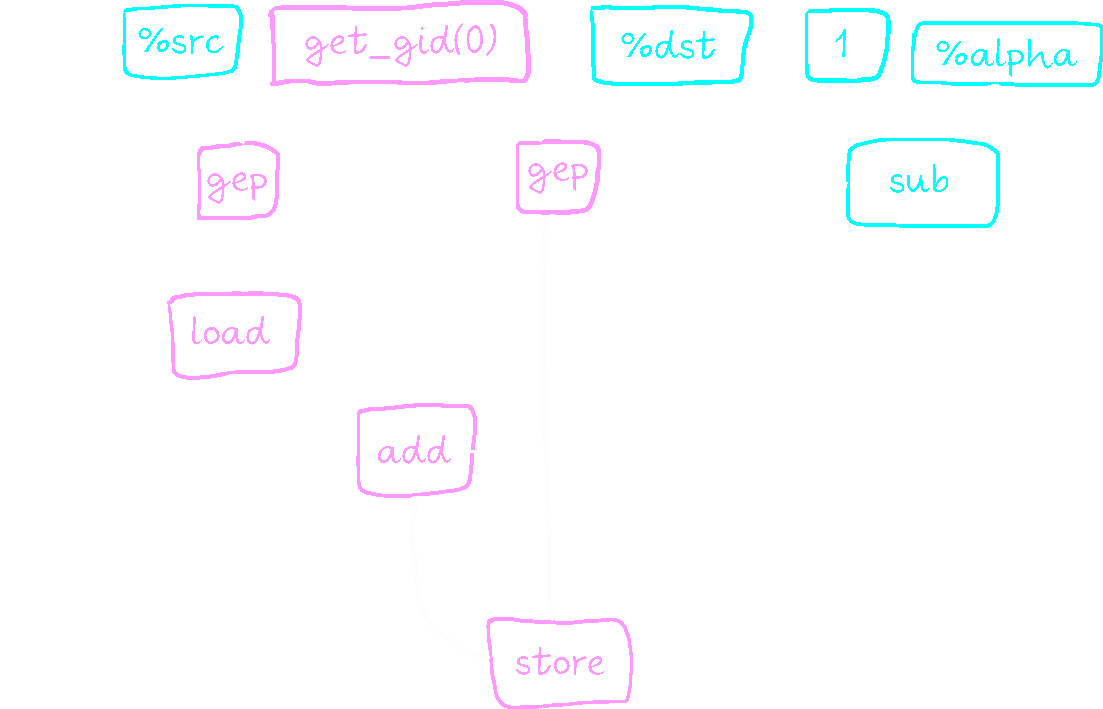
\includegraphics[scale=0.55]{images/packetization-2.pdf}}

\end{frame}

%%%%%%%%%%%%%%%%%%%%%%%%%%%%%%%%%%%%%%%%%%%%%%%%%%%%%%%%%%%%%%%%%%%%%%%%%%%%%%%%

\begin{frame}[c]{Packetization Example}

\center{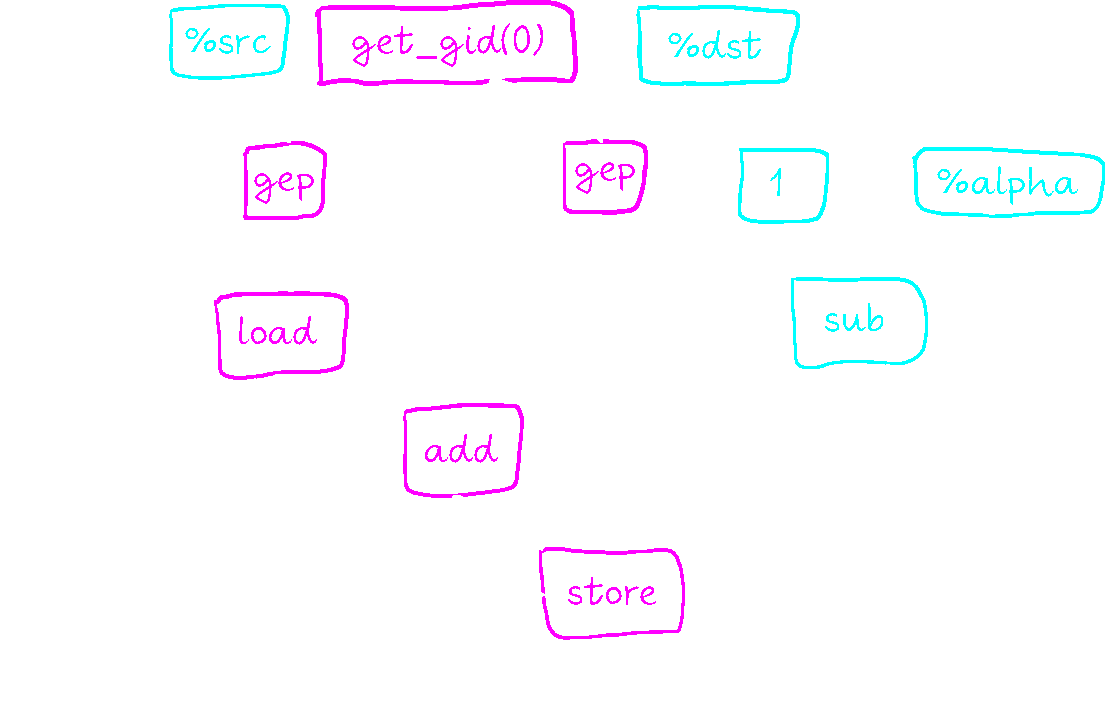
\includegraphics[scale=0.55]{images/packetization-3.pdf}}

\end{frame}

%%%%%%%%%%%%%%%%%%%%%%%%%%%%%%%%%%%%%%%%%%%%%%%%%%%%%%%%%%%%%%%%%%%%%%%%%%%%%%%%

\begin{frame}[c]{Packetization Example}

\center{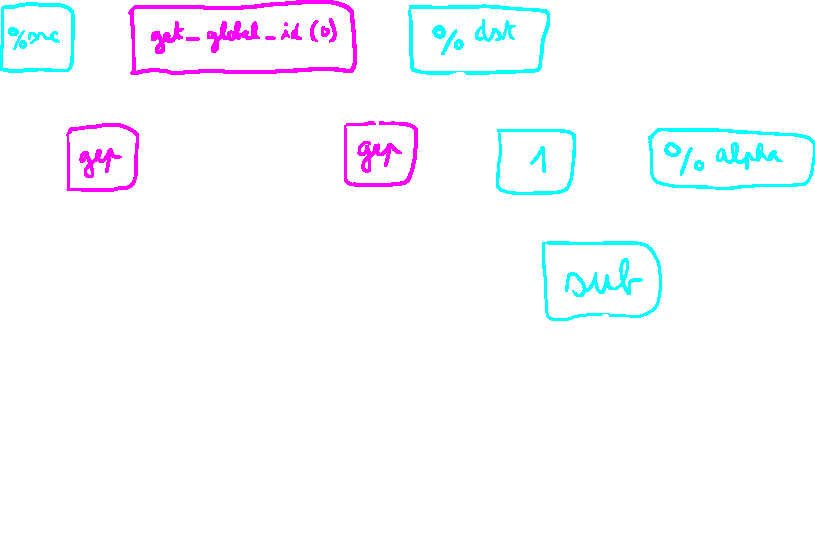
\includegraphics[scale=0.55]{images/packetization-4.pdf}}

\end{frame}

%%%%%%%%%%%%%%%%%%%%%%%%%%%%%%%%%%%%%%%%%%%%%%%%%%%%%%%%%%%%%%%%%%%%%%%%%%%%%%%%

\begin{frame}[fragile]{Packetization Example}

\begin{codebox}[commandchars=\\\[\]]
define void @__v4_add_uniform(i32* \uniform[%dst], i32* \uniform[%src], i32 \uniform[%alpha]) {
entry:
  \varying[%tid] = call i32 \varying[@get_global_id(i32 0)]
  \varying[%arrayidx] = getelementptr i32* \uniform[%src], i32 \varying[%tid]
  \varying[%0] = bitcast i32* \varying[%arrayidx] to <4 x i32>*
  \varying[%1] = load <4 x i32>* \varying[%0], align 4

  ; Broadcast (alpha - 1) to a vector
  \uniform[%sub] = sub i32 \uniform[%alpha], \uniform[1]
  \uniform[%insert] = insertelement <4 x i32> undef, i32 \uniform[%sub], i32 0
  \uniform[%broadcast_sub] = shufflevector <4 x i32> \uniform[%insert], ...

  \varying[%add] = add nsw <4 x i32> \uniform[%broadcast_sub], \varying[%1]

  \varying[%arrayidx2] = getelementptr i32* \uniform[%dst], i32 \varying[%tid]
  \varying[%2] = bitcast i32* \varying[%arrayidx2] to <4 x i32>*
  store <4 x i32> \varying[%add], <4 x i32>* \varying[%2], align 4
  ret void
}
\end{codebox}

\end{frame}

\talksection{Scalarization Stage}

\begin{frame}[fragile]{Scalarization Overview}

\begin{itemize}
    \item Eliminates vector operations from the source function
    \item Vector types used likely to be narrower than the native SIMD width
    \item Combining scalarization with packetization
    \begin{itemize}
        \item Generate vector instructions with the native SIMD width
        \item Implicitely performs 'Structure-of-Arrays to Array-of-Structures' conversion
    \end{itemize}
    \item Alternative is instantiating vector instructions (and users) $N$ times
    \item Example: Extract audio samples  from left and right channels, scale by $\frac{1}{2}$
\end{itemize}

\begin{codebox}[commandchars=\\\[\]]
global int2 \uniform[*src], int \uniform[*left], int \uniform[*right];
int \varying[tid] = \varying[get_global_id(0)];
int2 \varying[sample] = \uniform[src]\idx[\varying[tid]];
\uniform[left]\idx[\varying[tid]] = (\varying[sample.x] >> \uniform[1]);
\uniform[right]\idx[\varying[tid]] = (\varying[sample.y] >> \uniform[1]);
\end{codebox}

\end{frame}

%%%%%%%%%%%%%%%%%%%%%%%%%%%%%%%%%%%%%%%%%%%%%%%%%%%%%%%%%%%%%%%%%%%%%%%%%%%%%%%%

\begin{frame}{Scalarization Process}

\begin{itemize}
    \item Look for vector \varying{varying} instructions such as:
    \begin{itemize}
        \item Leaves that define vector values, vector stores
        \item Vector extractions
        \item Vector -> scalar bitcasts
    \end{itemize}
    
    \item Recursively scalarize until we reach a scalar value
    \begin{itemize}
        \item Operands before instructions
        \item Re-create instructions for each vector element
        \item Vector lane $\neq$ SIMD instance!
    \end{itemize}
    
\end{itemize}

\end{frame}

%%%%%%%%%%%%%%%%%%%%%%%%%%%%%%%%%%%%%%%%%%%%%%%%%%%%%%%%%%%%%%%%%%%%%%%%%%%%%%%%

\begin{frame}[c]{Scalarization Example: Before}

\center{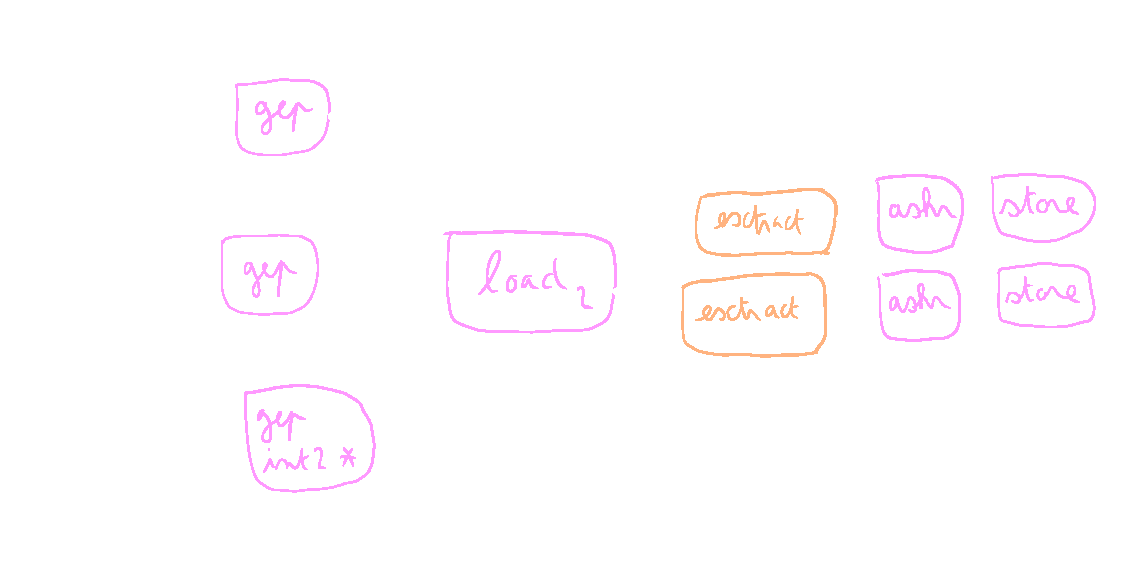
\includegraphics[scale=0.65]{images/scalarization-start.pdf}}

\end{frame}

%%%%%%%%%%%%%%%%%%%%%%%%%%%%%%%%%%%%%%%%%%%%%%%%%%%%%%%%%%%%%%%%%%%%%%%%%%%%%%%%

\begin{frame}{Scalarization Example: After}

[ IR Graph After ]

\end{frame}

%%%%%%%%%%%%%%%%%%%%%%%%%%%%%%%%%%%%%%%%%%%%%%%%%%%%%%%%%%%%%%%%%%%%%%%%%%%%%%%%

\begin{frame}[fragile]{Scalarization Example: IR}

Before Scalarization:
\begin{codebox}
kernel void extract_lr(global int2 *src, global int *left, global int *right) {
    int tid = get_global_id(0);
    int2 sample = src[tid];
    left[tid] = (sample.x >> 1);
    right[tid] = (sample.y >> 1);
}
\end{codebox}

After Scalarization:
\begin{codebox}
kernel void extract_lr(global int2 *src, global int *left, global int *right) {
    int tid = get_global_id(0);
    int sampleLeft = *((int *)&src[tid] + 0);
    int sampleRight = *((int *)&src[tid] + 1);
    left[tid] = (sampleLeft >> 1);
    right[tid] = (sampleRight >> 1);
}
\end{codebox}

\end{frame}

%%%%%%%%%%%%%%%%%%%%%%%%%%%%%%%%%%%%%%%%%%%%%%%%%%%%%%%%%%%%%%%%%%%%%%%%%%%%%%%%

\begin{frame}[fragile]{Scalarization Example}

After Scalarization:
\begin{codebox}
kernel void extract_lr(global int2 *src, global int *left, global int *right) {
    int tid = get_global_id(0);
    int sampleLeft = *((int *)&src[tid] + 0);
    int sampleRight = *((int *)&src[tid] + 1);
    left[tid] = (sampleLeft >> 1);
    right[tid] = (sampleRight >> 1);
}
\end{codebox}

After Packetization:
\begin{codebox}
kernel void extract_lr(global int2 *src, global int *left, global int *right) {
    int tid = get_global_id(0);
    int4 samplesLeft  = interleaved_load_int4((int *)&src[tid] + 0, 2);
    int4 samplesRight = interleaved_load_int4((int *)&src[tid] + 1, 2);
    ((int4 *)left)[tid / 4] = (samplesLeft >> 1);
    ((int4 *)right)[tid / 4] = (samplesRight >> 1);
}
\end{codebox}

\end{frame}

\talksection{Control Flow Conversion Stage}

\begin{frame}{Control Flow Conversion: Overview}

\begin{itemize}
    \item Linearizes functions that have \varying{divergent} control flow
    \begin{itemize}
        \item Conversion from control flow to data flow
        \item All basic blocks are executed
        \item Program semantics are preserved using predication (masking)
    \end{itemize}
    \item Why is it needed?
    \begin{itemize}
        \item SIMD unit does not support 'vector' (\varying{divergent}) branches
        \item Single program counter per SIMD group
    \end{itemize}
    \item Requires some passes to be run in the 'Prepare' stage
    \begin{itemize}
        \item Functions should have a single return block
        \item Loops should be in 'simple form'
    \end{itemize}
\end{itemize}

\vfill
\hspace{1em}
\includegraphics[scale=0.55]{images/stages-control-flow.pdf}

\end{frame}

%%%%%%%%%%%%%%%%%%%%%%%%%%%%%%%%%%%%%%%%%%%%%%%%%%%%%%%%%%%%%%%%%%%%%%%%%%%%%%%%

\begin{frame}[fragile]{Control Flow Conversion: if}

\begin{minipage}[t]{0.50\linewidth}

\begin{itemize}
    \item Divergent branch condition: \varying{cond}
    \item Instruction with side-effects: \texttt{load}
\end{itemize}

\begin{codebox}[commandchars=\\\[\]]
kernel void copy_if_even(global int \uniform[*src],
                         global int \uniform[*dst]) {
  int \varying[tid] = \varying[get_global_id(0)];
  int \varying[cond] = (\varying[tid] & \uniform[1]) == \uniform[0];
  int result;
  if (\varying[cond]) {
    \varying[result] = \uniform[src]\idx[\varying[tid]];
  } else {
    \uniform[result] = \uniform[-1];
  }
  \uniform[dst]\idx[\varying[tid]] = \varying[result];
}
\end{codebox}

\end{minipage}
\hspace{1em}
\begin{minipage}[t]{0.43\linewidth}

\vspace{0.1ex}

\center{
\includegraphics[scale=0.45]{images/if-cfg.pdf}}

\end{minipage}

\end{frame}

%%%%%%%%%%%%%%%%%%%%%%%%%%%%%%%%%%%%%%%%%%%%%%%%%%%%%%%%%%%%%%%%%%%%%%%%%%%%%%%%

\begin{frame}{Control Flow Conversion: Main Steps}

\begin{itemize}
    \item Divergence Analysis
    \item Generate Masks
    \item Freeze Loop Live Variables
    \item Apply Masks
    \begin{itemize}
        \item Instructions with side-effects
    \end{itemize}
    \item Convert Phi Nodes
    \begin{itemize}
        \item Preserves data flow
    \end{itemize}
    \item CFG Linearization
    %\begin{itemize}
    %    \item Flattens the Control Flow Graph
    %\end{itemize}
\end{itemize}

\end{frame}

%%%%%%%%%%%%%%%%%%%%%%%%%%%%%%%%%%%%%%%%%%%%%%%%%%%%%%%%%%%%%%%%%%%%%%%%%%%%%%%%

\begin{frame}{CFG Linearization Overview}

\begin{minipage}[t]{0.45\linewidth}

\begin{itemize}
    \item Flattens the CFG
    \begin{itemize}
        \item All blocks are executed
        \item Regardless of branch conditions
    \end{itemize}
    %\item Masks and selects take care of preserving the data flow
    \item Steps
    \begin{itemize}
        \item Order blocks
        \item Rewrite branches
    \end{itemize}
    \item More on this later
\end{itemize}

\end{minipage}
\hspace{1em}
\begin{minipage}[t]{0.43\linewidth}

\vspace{0.1ex}

\center{
\includegraphics[scale=0.35]{images/linearization-overview.pdf}}

\end{minipage}

\end{frame}

%%%%%%%%%%%%%%%%%%%%%%%%%%%%%%%%%%%%%%%%%%%%%%%%%%%%%%%%%%%%%%%%%%%%%%%%%%%%%%%%

\begin{frame}{Basic Divergence Analysis}

\begin{minipage}[t]{0.50\linewidth}

\begin{itemize}
    \item Determines which basic blocks need predication (i.e. are \varying{divergent})
    \item BB is \varying{divergent} if:
    \begin{itemize}
        \item Any predecessor has a branch with a \varying{varying} condition
        \item Any predecessor is \varying{divergent} (naive)
    \end{itemize}
    \item Process:
    \begin{itemize}
        \item Start with the entry BB
        \item Mark successors \varying{divergent} or not
        \item Visit all successors recursively
        \item Visit each BB only once (cycles)
    \end{itemize}
\end{itemize}

\end{minipage}
\hspace{1em}
\begin{minipage}[t]{0.43\linewidth}

\vspace{-2.1ex}
\center{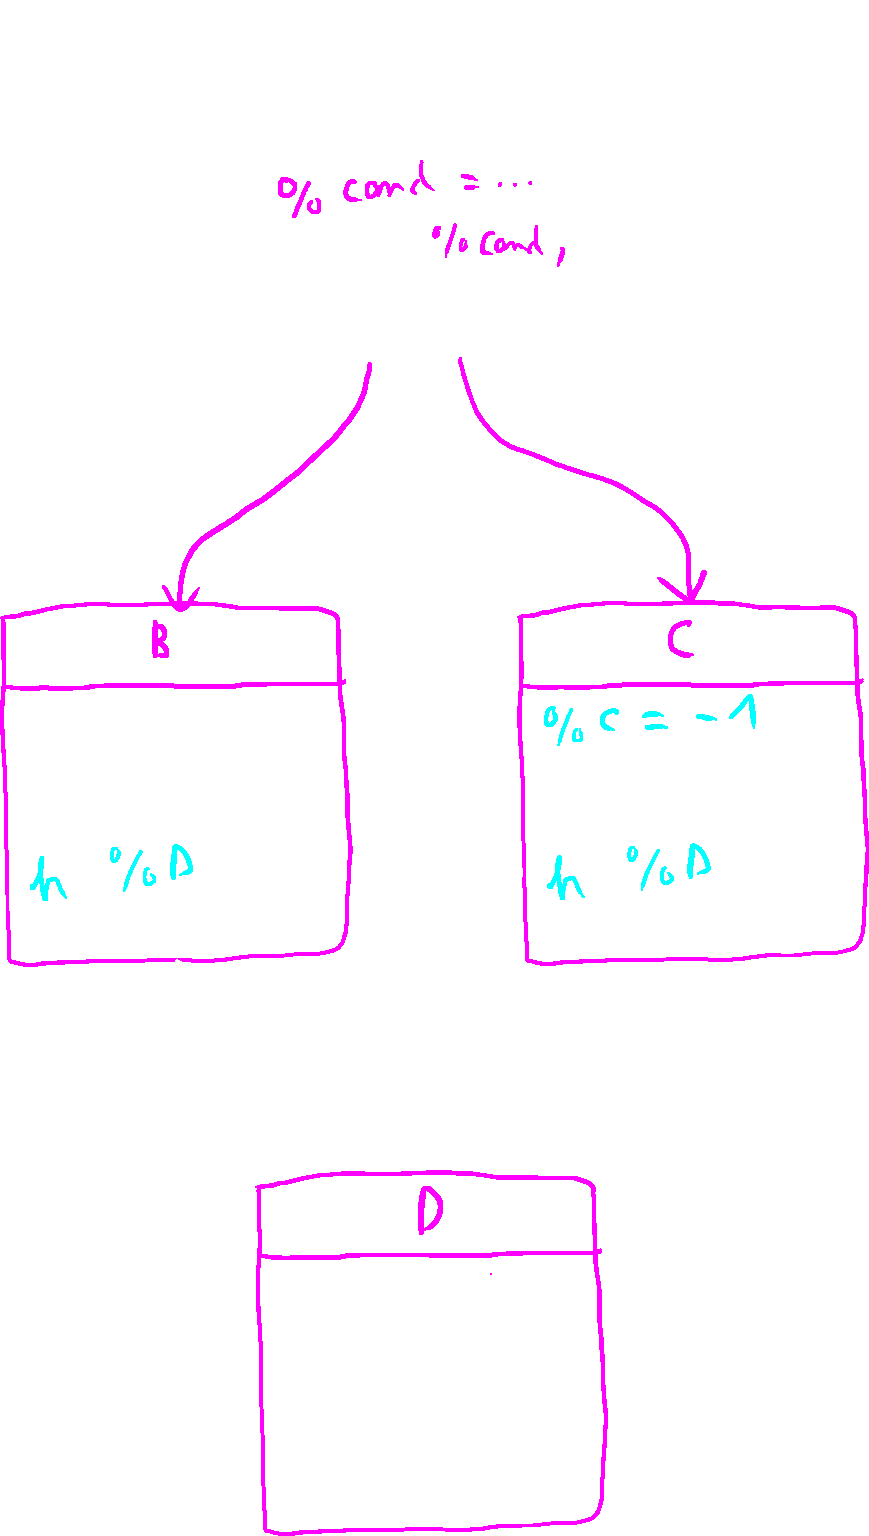
\includegraphics[scale=0.26]{images/divergence-analysis.pdf}}

\end{minipage}

\end{frame}

%%%%%%%%%%%%%%%%%%%%%%%%%%%%%%%%%%%%%%%%%%%%%%%%%%%%%%%%%%%%%%%%%%%%%%%%%%%%%%%%

\begin{frame}{Mask Generation}

\begin{minipage}[t]{0.50\linewidth}

\begin{itemize}
    \item Mask: $N$-bit field (1-bit pre-packetization)
    \begin{itemize}
        \item Per-instance, 'active' bit for predication
    \end{itemize}
    \item Each edge $A \rightarrow B$ has a mask: $m_{A \rightarrow B}$
    \begin{itemize}
        \item Which lanes take the branch to $B$?
        \item $m_{A \rightarrow B} = m_A \cap bcond_{A \rightarrow B}$
        \item Given branch condition $bcond_{A \rightarrow B}$
    \end{itemize}
    \item Each block $B$ has an entry mask: $m_B$
    \begin{itemize}
        \item Which lanes execute $B$?
        \item $m_B = \bigcup\limits_{i=0}^n  m_{P_i \rightarrow B}$
        \item Given predecessors $P_0$ $\cdots$ $P_n$
    \end{itemize}
    \item Start by generating return mask $m_D$
    \begin{itemize}
        \item Depends on all other masks
    \end{itemize}
\end{itemize}

\end{minipage}
\hspace{1em}
\begin{minipage}[t]{0.43\linewidth}

\vspace{-2.1ex}
\center{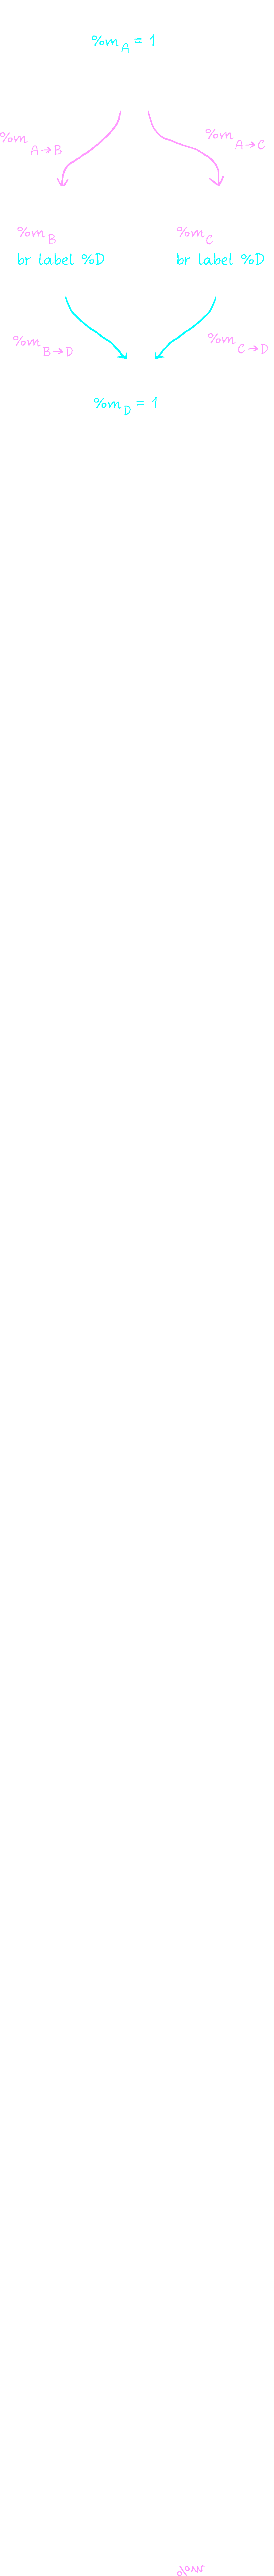
\includegraphics[scale=0.30]{images/mask-generation.pdf}}

\end{minipage}

\end{frame}

%%%%%%%%%%%%%%%%%%%%%%%%%%%%%%%%%%%%%%%%%%%%%%%%%%%%%%%%%%%%%%%%%%%%%%%%%%%%%%%%

\begin{frame}{Applying Masks}

\begin{itemize}
    \item Each block $B$ is executed regardless of whether $F$ executes it or not
    \item Each instruction $I$ that has side-effects need 'guarding'
    \item Such instructions are predicated using $m_B$
    \begin{itemize}
        \item $I$ has side-effects for lane $L$ if $m_B[L]$ is true
        \item Loads and stores are turned into masked loads and stores
        \item Calls to functions with side-effects: $m_B$ is passed as an argument
        \item Floating-point instructions that raise exceptions (e.g. DIV0)
        \item ...
    \end{itemize}
    \item Unsupported masked operations can be expanded
    \begin{itemize}
        \item For each lane $L$, generate: \texttt{if ($m_B[L]$) \{ $V_L=I_L(...)$; \}}
        \item Need to create many basic blocks
    \end{itemize}
\end{itemize}

\end{frame}

%%%%%%%%%%%%%%%%%%%%%%%%%%%%%%%%%%%%%%%%%%%%%%%%%%%%%%%%%%%%%%%%%%%%%%%%%%%%%%%%

\begin{frame}[fragile]{Phi Conversion}

\begin{itemize}
    \item A phi node:
    \begin{itemize}
        \item Takes incoming blocks $P_0 \cdots P_n$, values $V_0 \cdots V_n$
        \item Evaluates to $V_i$ if the incoming block was $P_i$
    \end{itemize}
    \item Does not work after linearization
    \begin{itemize}
        \item Each block $B$ has a single predecessor after linearization
        %\item Actual incoming block encoded by $m_{P_0 \rightarrow B} \cdots m_{P_n \rightarrow B}$
        \item Actual incoming block: find $P_i$, so that $m_{P_i \rightarrow B}$ is true
    \end{itemize}
    \item Need to convert phi nodes into $n$ select instructions
    \begin{itemize}
        \item Using $m_{P_0 \rightarrow B} \cdots m_{P_n \rightarrow B}$ to select $V$ from $V_0 \cdots V_n$
    \end{itemize}
\end{itemize}

\hspace{3.0em}\begin{minipage}[t]{0.38\linewidth}

\begin{codebox}[commandchars=\\\[\]]
A:
  \varying[%cmp] = ...
  br i1 \varying[%cmp], label %B, label %C
B:
  \varying[%x] = load i32* \varying[%idx]
  br label %C
C:
  \varying[%v] = phi i32 \idx[\varying[%x], %B], \idx[\uniform[-1], %A]
\end{codebox}

\end{minipage}\hspace{1em}\begin{minipage}[t]{0.42\linewidth}

\begin{codebox}[commandchars=\\\[\]]
A:
  \varying[%cmp] = ... // = mAB = mB = mBC
  br label %B
B:
  \varying[%x] = masked_load i32* \varying[%idx], i1 \varying[%cmp]
  br label %C
C:
  \varying[%v] = select i1 \varying[%cmp], i32 \varying[%x], i32 \uniform[-1]
\end{codebox}

\end{minipage}

\end{frame}

%%%%%%%%%%%%%%%%%%%%%%%%%%%%%%%%%%%%%%%%%%%%%%%%%%%%%%%%%%%%%%%%%%%%%%%%%%%%%%%%

\begin{frame}[fragile]{CFG Conversion Result: if}

\begin{codebox}
define void @__v4_copy_if_eveni(i32* %in, i32* %out) {
entry:
  %call = call spir_func i64 @get_global_id(i32 0)
  %.splatinsert = insertelement <4 x i64> undef, i64 %call, i32 0
  %.splat = shufflevector <4 x i64> %.splatinsert, <4 x i64> undef, <4 x i32> zeroinit
  %0 = add <4 x i64> %.splat, <i64 0, i64 1, i64 2, i64 3>
  %and1 = and <4 x i64> %0, <i64 1, i64 1, i64 1, i64 1>
  %cmp2 = icmp eq <4 x i64> %and1, zeroinitializer

; if.then:
  %arrayidx = getelementptr inbounds i32* %in, i64 %call
  %1 = call <4 x i32> @masked_load4(i32* %arrayidx, <4 x i1> %cmp2)

; if.end:
  %2 = select <4 x i1> %cmp2, <4 x i32> %1, <4 x i32> <i32 -1, i32 -1, i32 -1, i32 -1>
  %arrayidx1 = getelementptr inbounds i32* %out, i64 %call
  %3 = bitcast i32* %arrayidx1 to <4 x i32>*
  store <4 x i32> %2, <4 x i32>* %3, align 4
  ret void
}
\end{codebox}

\end{frame}

%%%%%%%%%%%%%%%%%%%%%%%%%%%%%%%%%%%%%%%%%%%%%%%%%%%%%%%%%%%%%%%%%%%%%%%%%%%%%%%%

\begin{frame}[fragile]{Control Flow Conversion: Loops}

\begin{minipage}[t]{0.45\linewidth}

\begin{itemize}
    \item More difficult to convert
    %\begin{itemize}
    %    \item Need to keep iterating as long as any instance is inside the loop
    %    \item Need to freeze live variables
    %\end{itemize}
    \item More masks to compute
    \item Loop condition may be \varying{varying}
    %\begin{itemize}
    %    \item Exit mask
    %    \item Active mask
    %\end{itemize}
\end{itemize}

\begin{codebox}[commandchars=\\\[\]]
kernel void while_loop(global int \uniform[*src],
                       global int \uniform[*dst],
                       int \uniform[step]) {
  int \varying[tid] = \varying[get_global_id(0)];
  int \varying[val] = \uniform[src]\idx[\varying[tid]];
  while (\varying[val] < \uniform[0]) {
    \varying[val] += \uniform[step];
  }
  dst\idx[\varying[tid]] = \varying[val];
}
\end{codebox}

\end{minipage}
\hspace{1em}
\begin{minipage}[t]{0.43\linewidth}

\vspace{0.1ex}

\center{
\includegraphics[scale=0.60]{images/loop-example1.pdf}}

\end{minipage}

\end{frame}

%%%%%%%%%%%%%%%%%%%%%%%%%%%%%%%%%%%%%%%%%%%%%%%%%%%%%%%%%%%%%%%%%%%%%%%%%%%%%%%%

\begin{frame}{Loop Exit and Active Masks}

\begin{minipage}[t]{0.70\linewidth}

\begin{itemize}
    \item Different instances may iterate a different number of times
    \begin{itemize}
        \item Because the loop condition is \varying{varying}
        \item Keep iterating as long as any instance is inside the loop
    \end{itemize}
    \item Loop Exit mask $m_{Exit}$
    \begin{itemize}
        \item Keeps track of which instances exited the loop
        \item Used as entry mask for loop exits
        \item Used to freeze live variables
        \item Needs a phi node since this changes over iterations
    \end{itemize}
    \item Loop Active mask $m_{Active}$
    \begin{itemize}
        \item $m_{Active} = m_{Header} \cap \overline{m_{Exit}}$
        \item True: Branch from loop latch $L$ back to loop header $H$
        \item False: Exit the loop from loop latch $L$
    \end{itemize}
\end{itemize}

\end{minipage}
\hspace{1em}
\begin{minipage}[t]{0.23\linewidth}

\vspace{0.1ex}

\center{
\includegraphics[scale=0.60]{images/loop-linear-cfg.pdf}}

\end{minipage}

\end{frame}

%%%%%%%%%%%%%%%%%%%%%%%%%%%%%%%%%%%%%%%%%%%%%%%%%%%%%%%%%%%%%%%%%%%%%%%%%%%%%%%%

\begin{frame}{Freezing Loop Live Variables}

\begin{itemize}
    \item Variables that are either:
    \begin{itemize}
        \item Used in a subsequent loop iteration (through a phi node)
        \item Used outside of the loop
        \item In the example: \varying{val}
    \end{itemize}
    \item Once an instance exits, need to freeze live variables
    \begin{itemize}
        \item Otherwise will have the wrong value after the loop 
    \end{itemize}
    \item Create a select that returns either: 
    \begin{itemize}
        \item The value from the previous iteration (instance exited)
        \item The new value from this iteration (instance still active)
    \end{itemize}
    \item The Loop Exit mask selects the right value
    \item Replace all uses of the new value with the select
\end{itemize}

\end{frame}

%%%%%%%%%%%%%%%%%%%%%%%%%%%%%%%%%%%%%%%%%%%%%%%%%%%%%%%%%%%%%%%%%%%%%%%%%%%%%%%%

\begin{frame}{Basic Linearization: Graph Creation}

\begin{itemize}
    \item Create a CFG-like graph
    \begin{itemize}
        \item Where a loop's blocks are replaced by a single loop node
        \item The loop node (\codeemphb{S}) contains a sub-graph
    \end{itemize}
    \item Sub-graphs can contain blocks and loops
    \begin{itemize}
        \item Allows recursive processing of loop nests
    \end{itemize}
\end{itemize}

\center{
\includegraphics[scale=0.50]{images/loop-linearization1.pdf}}

\end{frame}

%%%%%%%%%%%%%%%%%%%%%%%%%%%%%%%%%%%%%%%%%%%%%%%%%%%%%%%%%%%%%%%%%%%%%%%%%%%%%%%%

\begin{frame}{Basic Linearization: Block Ordering}

\begin{minipage}[t]{0.50\linewidth}

\begin{itemize}
    \item Bottom-up topological sort of the graph
    \begin{itemize}
        \item Result is an ordered list of graph nodes
        \item Loop nodes expand to sub-lists
        \item Topological sort of loop nodes starts at the loop latch
    \end{itemize}
    \item Naive approach that linearizes everything
\end{itemize}

\end{minipage}
\hspace{1em}
\begin{minipage}[t]{0.38\linewidth}

\vspace{0.1ex}

\center{
\includegraphics[scale=0.50]{images/loop-linearization2.pdf}}

\end{minipage}

\end{frame}

%%%%%%%%%%%%%%%%%%%%%%%%%%%%%%%%%%%%%%%%%%%%%%%%%%%%%%%%%%%%%%%%%%%%%%%%%%%%%%%%

\begin{frame}{Basic Linearization: Branch Rewriting}

\begin{minipage}[t]{0.55\linewidth}

\begin{itemize}
    \item Visit each block in the ordered list
    \item Rewrite their branch target
\end{itemize}

\begin{itemize}
    \item For most blocks:
    \begin{itemize}
        \item Always branch to the next block in the list
    \end{itemize}
    \item For the loop latch $L$:
    \begin{itemize}
        \item How many active instances in the loop?
        \item $\geq 1$: Branch to the loop header $H$
        \item $0$: Branch to next block
        \item Use the Loop Active mask
    \end{itemize}
\end{itemize}

\end{minipage}
\begin{minipage}[t]{0.42\linewidth}

\vspace{0.1ex}

\center{
\includegraphics[scale=0.45]{images/loop-linearization3.pdf}}

\end{minipage}

\end{frame}

%%%%%%%%%%%%%%%%%%%%%%%%%%%%%%%%%%%%%%%%%%%%%%%%%%%%%%%%%%%%%%%%%%%%%%%%%%%%%%%%


%\talkpart{3}{Going Further}
%%%%%%%%%%%%%%%%%%%%%%%%%%%%%%%%%%%%%%%%%%%%%%%%%%%%%%%%%%%%%%%%%%%%%%%%%%%%%%%%%

\begin{frame}{SIMD width detection}

\end{frame}

%%%%%%%%%%%%%%%%%%%%%%%%%%%%%%%%%%%%%%%%%%%%%%%%%%%%%%%%%%%%%%%%%%%%%%%%%%%%%%%%

\begin{frame}{Vectorizing builtin function calls}

% Builtin: the vectorizer has some knowledge of scalar -> vector function mapping

\end{frame}

%%%%%%%%%%%%%%%%%%%%%%%%%%%%%%%%%%%%%%%%%%%%%%%%%%%%%%%%%%%%%%%%%%%%%%%%%%%%%%%%

\begin{frame}{Vectorizing builtin functions}

% By vectorizing the builtin's body
% This changes the function signature (return value, some arguments)
% Builtin: the vectorizer has some knowledge of which arguments need packetization
% Need argument placeholders (cloning required)
% Packetized arguments are roots (Uniform Value Analysis)
% Return instructions are leaves (Packetization Stage)

\end{frame}

%%%%%%%%%%%%%%%%%%%%%%%%%%%%%%%%%%%%%%%%%%%%%%%%%%%%%%%%%%%%%%%%%%%%%%%%%%%%%%%%

\begin{frame}{Vectorizing user functions (no side effects)}

% Similar to builtin functions, but with no knowledge of whether arguments need
% packetization. Need to analyze this for each call site.

\end{frame}

%%%%%%%%%%%%%%%%%%%%%%%%%%%%%%%%%%%%%%%%%%%%%%%%%%%%%%%%%%%%%%%%%%%%%%%%%%%%%%%%

\begin{frame}{Vectorizing user functions (with side effects)}

% Need to pass a mask as an extra argument
% Might be simpler to just inline such functions

\end{frame}

%%%%%%%%%%%%%%%%%%%%%%%%%%%%%%%%%%%%%%%%%%%%%%%%%%%%%%%%%%%%%%%%%%%%%%%%%%%%%%%%

\begin{frame}{Interleaved memory optimizations}

\end{frame}

%%%%%%%%%%%%%%%%%%%%%%%%%%%%%%%%%%%%%%%%%%%%%%%%%%%%%%%%%%%%%%%%%%%%%%%%%%%%%%%%

\begin{frame}{SoA to AoS conversion}

\end{frame}




%%%%%%%%%%%%%%%%%%%%%%%%%%%%%%%%%%%%%%%%%%%%%%%%%%%%%%%%%%%%%%%%%%%%%%%%%%%%%%%%

\section*{Conclusion}

\begin{frame}{Conclusion}

\begin{itemize}
    \item Explained basic concepts
    \begin{itemize}
        \item Data-parallel execution model
        \item Whole-function vectorization
        \item $N$ instances of every instruction
        \item \uniform{Uniform} vs \varying{varying} values
        \item \varying{Divergent} control flow, masking
    \end{itemize}
    \item Many things were not covered in this talk
    \begin{itemize}
        \item Loops with multiple exits
        \item More advanced analyses
        \item Optimizations
        \item ...
    \end{itemize}
    \item Should be enough to create a functional vectorizer
\end{itemize}

\end{frame}

%%%%%%%%%%%%%%%%%%%%%%%%%%%%%%%%%%%%%%%%%%%%%%%%%%%%%%%%%%%%%%%%%%%%%%%%%%%%%%%%

\begin{frame}{References and Resources}

\begin{itemize}
    \item Automatic Packetization [Ralf Karrenberg, Saarland University '09]
    \item Whole-Function Vectorization (Ralf Karrenberg, Sebastian Hack, CGO '11)
    \item Intel\textregistered \, OpenCL\textsuperscript{TM} Implicit Vectorization Module [Nadav Rotem, LLVM '11]
    %\item Improving Performance of OpenCL on CPUs [Ralf Karrenberg et al., EuroLLVM '12]
    \item Branching in Data-Parallel Languages using Predication with LLVM [Marcello Maggioni, EuroLLVM '14]
    \item Exploring the Design Space of SPMD Divergence Management on Data-Parallel Architectures [Yunsup Lee et al., MICRO '14]
\end{itemize}

\vspace{11ex}

\footnotesize{OpenCL and the OpenCL logo are trademarks of Apple Inc. used by permission by Khronos.}

\vspace{1ex}\footnotesize{CUDA is a trademark and/or registered trademark of NVIDIA Corporation in the U.S. and/or other countries.}

\end{frame}

%%%%%%%%%%%%%%%%%%%%%%%%%%%%%%%%%%%%%%%%%%%%%%%%%%%%%%%%%%%%%%%%%%%%%%%%%%%%%%%%

\begin{frame}{Thank you!}

\begin{itemize}
    \item Q\&A
    \begin{itemize}
        \item Happy to answer questions by email too: \codeemphb{pierre-andre@codeplay.com}
    \end{itemize}
    \item ...
    \item Happy vectorizing!
\end{itemize}

%\vspace{2em}
%\center{\huge<\llvmlogovec{0.040}}
\center{\huge<\llvmlogovec{0.040},}
\center{\hspace{2.5em}\huge\llvmlogovec{0.040}>}

\end{frame}

%%%%%%%%%%%%%%%%%%%%%%%%%%%%%%%%%%%%%%%%%%%%%%%%%%%%%%%%%%%%%%%%%%%%%%%%%%%%%%%%

\talkpartslide{3}{Going Further}
%%%%%%%%%%%%%%%%%%%%%%%%%%%%%%%%%%%%%%%%%%%%%%%%%%%%%%%%%%%%%%%%%%%%%%%%%%%%%%%%

\begin{frame}{SIMD width detection}

\end{frame}

%%%%%%%%%%%%%%%%%%%%%%%%%%%%%%%%%%%%%%%%%%%%%%%%%%%%%%%%%%%%%%%%%%%%%%%%%%%%%%%%

\begin{frame}{Vectorizing builtin function calls}

% Builtin: the vectorizer has some knowledge of scalar -> vector function mapping

\end{frame}

%%%%%%%%%%%%%%%%%%%%%%%%%%%%%%%%%%%%%%%%%%%%%%%%%%%%%%%%%%%%%%%%%%%%%%%%%%%%%%%%

\begin{frame}{Vectorizing builtin functions}

% By vectorizing the builtin's body
% This changes the function signature (return value, some arguments)
% Builtin: the vectorizer has some knowledge of which arguments need packetization
% Need argument placeholders (cloning required)
% Packetized arguments are roots (Uniform Value Analysis)
% Return instructions are leaves (Packetization Stage)

\end{frame}

%%%%%%%%%%%%%%%%%%%%%%%%%%%%%%%%%%%%%%%%%%%%%%%%%%%%%%%%%%%%%%%%%%%%%%%%%%%%%%%%

\begin{frame}{Vectorizing user functions (no side effects)}

% Similar to builtin functions, but with no knowledge of whether arguments need
% packetization. Need to analyze this for each call site.

\end{frame}

%%%%%%%%%%%%%%%%%%%%%%%%%%%%%%%%%%%%%%%%%%%%%%%%%%%%%%%%%%%%%%%%%%%%%%%%%%%%%%%%

\begin{frame}{Vectorizing user functions (with side effects)}

% Need to pass a mask as an extra argument
% Might be simpler to just inline such functions

\end{frame}

%%%%%%%%%%%%%%%%%%%%%%%%%%%%%%%%%%%%%%%%%%%%%%%%%%%%%%%%%%%%%%%%%%%%%%%%%%%%%%%%

\begin{frame}{Interleaved memory optimizations}

\end{frame}

%%%%%%%%%%%%%%%%%%%%%%%%%%%%%%%%%%%%%%%%%%%%%%%%%%%%%%%%%%%%%%%%%%%%%%%%%%%%%%%%

\begin{frame}{SoA to AoS conversion}

\end{frame}




%%%%%%%%%%%%%%%%%%%%%%%%%%%%%%%%%%%%%%%%%%%%%%%%%%%%%%%%%%%%%%%%%%%%%%%%%%%%%%%%

\begin{frame}{Implementation Strategy}

\begin{itemize}
    \item Create test kernels
    \begin{itemize}
        \item Start with very simple kernels (e.g. copy buffer, add two buffers)
        \item Gradually add more features (e.g. non-sequential memory accesses, vector instructions, etc)
    \end{itemize}
    
    \item Suggested implementation order
    \begin{itemize}
        \item Preparation and packetization first (required for simplest kernels)
        \item Then easier features: builtins, memory addressing, scalarization, instantiation
        \item More complex features last: control flow, optimizations
    \end{itemize}
\end{itemize}

\end{frame}

%%%%%%%%%%%%%%%%%%%%%%%%%%%%%%%%%%%%%%%%%%%%%%%%%%%%%%%%%%%%%%%%%%%%%%%%%%%%%%%%

\begin{frame}{Scalarization Process}

\begin{itemize}
    \item Look for vector \varying{varying} instructions such as:
    \begin{itemize}
        \item Leaves that define vector values, vector stores
        \item Vector extractions
        \item Vector -> scalar bitcasts
    \end{itemize}
    
    \item Recursively scalarize until we reach a scalar value
    \begin{itemize}
        \item Operands before instructions
        \item Re-create instructions for each vector element
        \item Vector lane $\neq$ SIMD instance!
    \end{itemize}
    
\end{itemize}

\end{frame}

%%%%%%%%%%%%%%%%%%%%%%%%%%%%%%%%%%%%%%%%%%%%%%%%%%%%%%%%%%%%%%%%%%%%%%%%%%%%%%%%

%\begin{frame}[c]{Scalarization Example: Before}
%
%\center{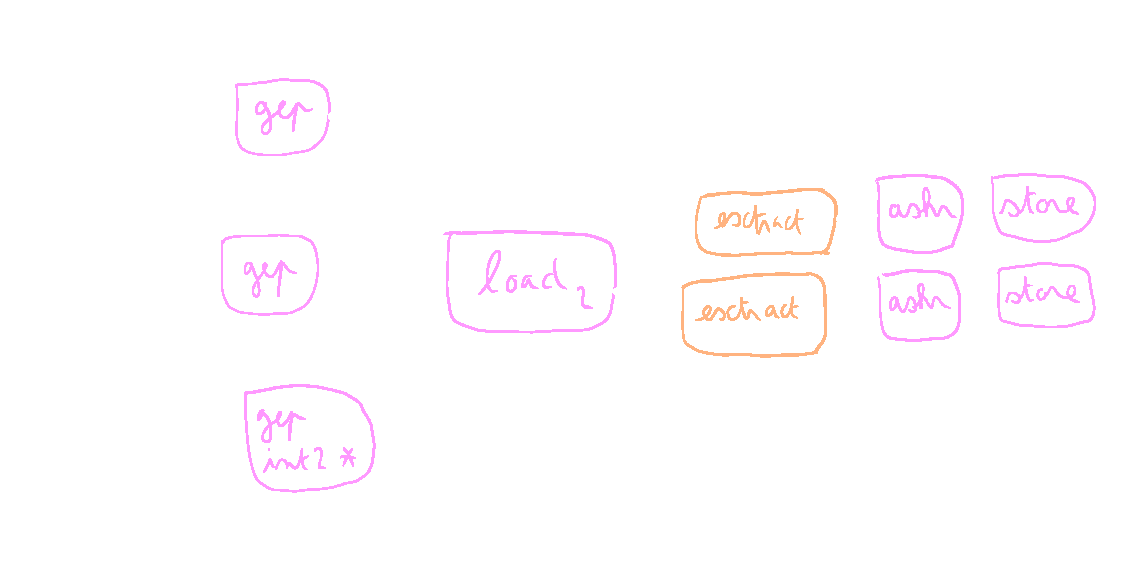
\includegraphics[scale=0.65]{images/scalarization-start.pdf}}
%
%\end{frame}

%%%%%%%%%%%%%%%%%%%%%%%%%%%%%%%%%%%%%%%%%%%%%%%%%%%%%%%%%%%%%%%%%%%%%%%%%%%%%%%%

%\begin{frame}{Scalarization Example: After}
%
%\center{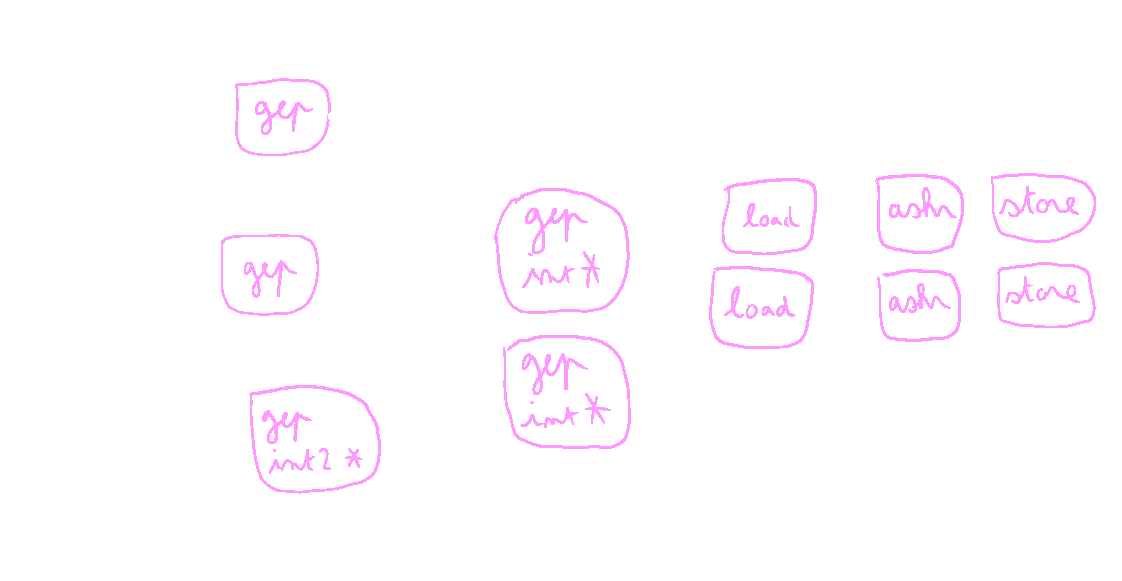
\includegraphics[scale=0.65]{images/scalarization-end.pdf}}
%
%\end{frame}

%%%%%%%%%%%%%%%%%%%%%%%%%%%%%%%%%%%%%%%%%%%%%%%%%%%%%%%%%%%%%%%%%%%%%%%%%%%%%%%%

\begin{frame}[fragile]{Scalarization Example}

After Scalarization:
\begin{codebox}
kernel void extract_lr(global int2 *src, global int *left, global int *right) {
    int tid = get_global_id(0);
    int sampleLeft = *((int *)&src[tid] + 0);
    int sampleRight = *((int *)&src[tid] + 1);
    left[tid] = (sampleLeft >> 1);
    right[tid] = (sampleRight >> 1);
}
\end{codebox}

After Packetization:
\begin{codebox}
kernel void extract_lr(global int2 *src, global int *left, global int *right) {
    int tid = get_global_id(0);
    int4 samplesLeft  = interleaved_load_int4((int *)&src[tid] + 0, 2);
    int4 samplesRight = interleaved_load_int4((int *)&src[tid] + 1, 2);
    ((int4 *)left)[tid / 4] = (samplesLeft >> 1);
    ((int4 *)right)[tid / 4] = (samplesRight >> 1);
}
\end{codebox}

\end{frame}


\end{document}
